\chapter{Results and Discussion}
\label{cha:3}

\section{Doping Characterization}

Upon increase of the dopant concentration that is deposited and bake on top of the p(g3T2-T) film, the reflection hue, as observed in Figure \ref{fig:color} shift towards more yellowish colors.

\begin{figure}[ht]
  \centering
  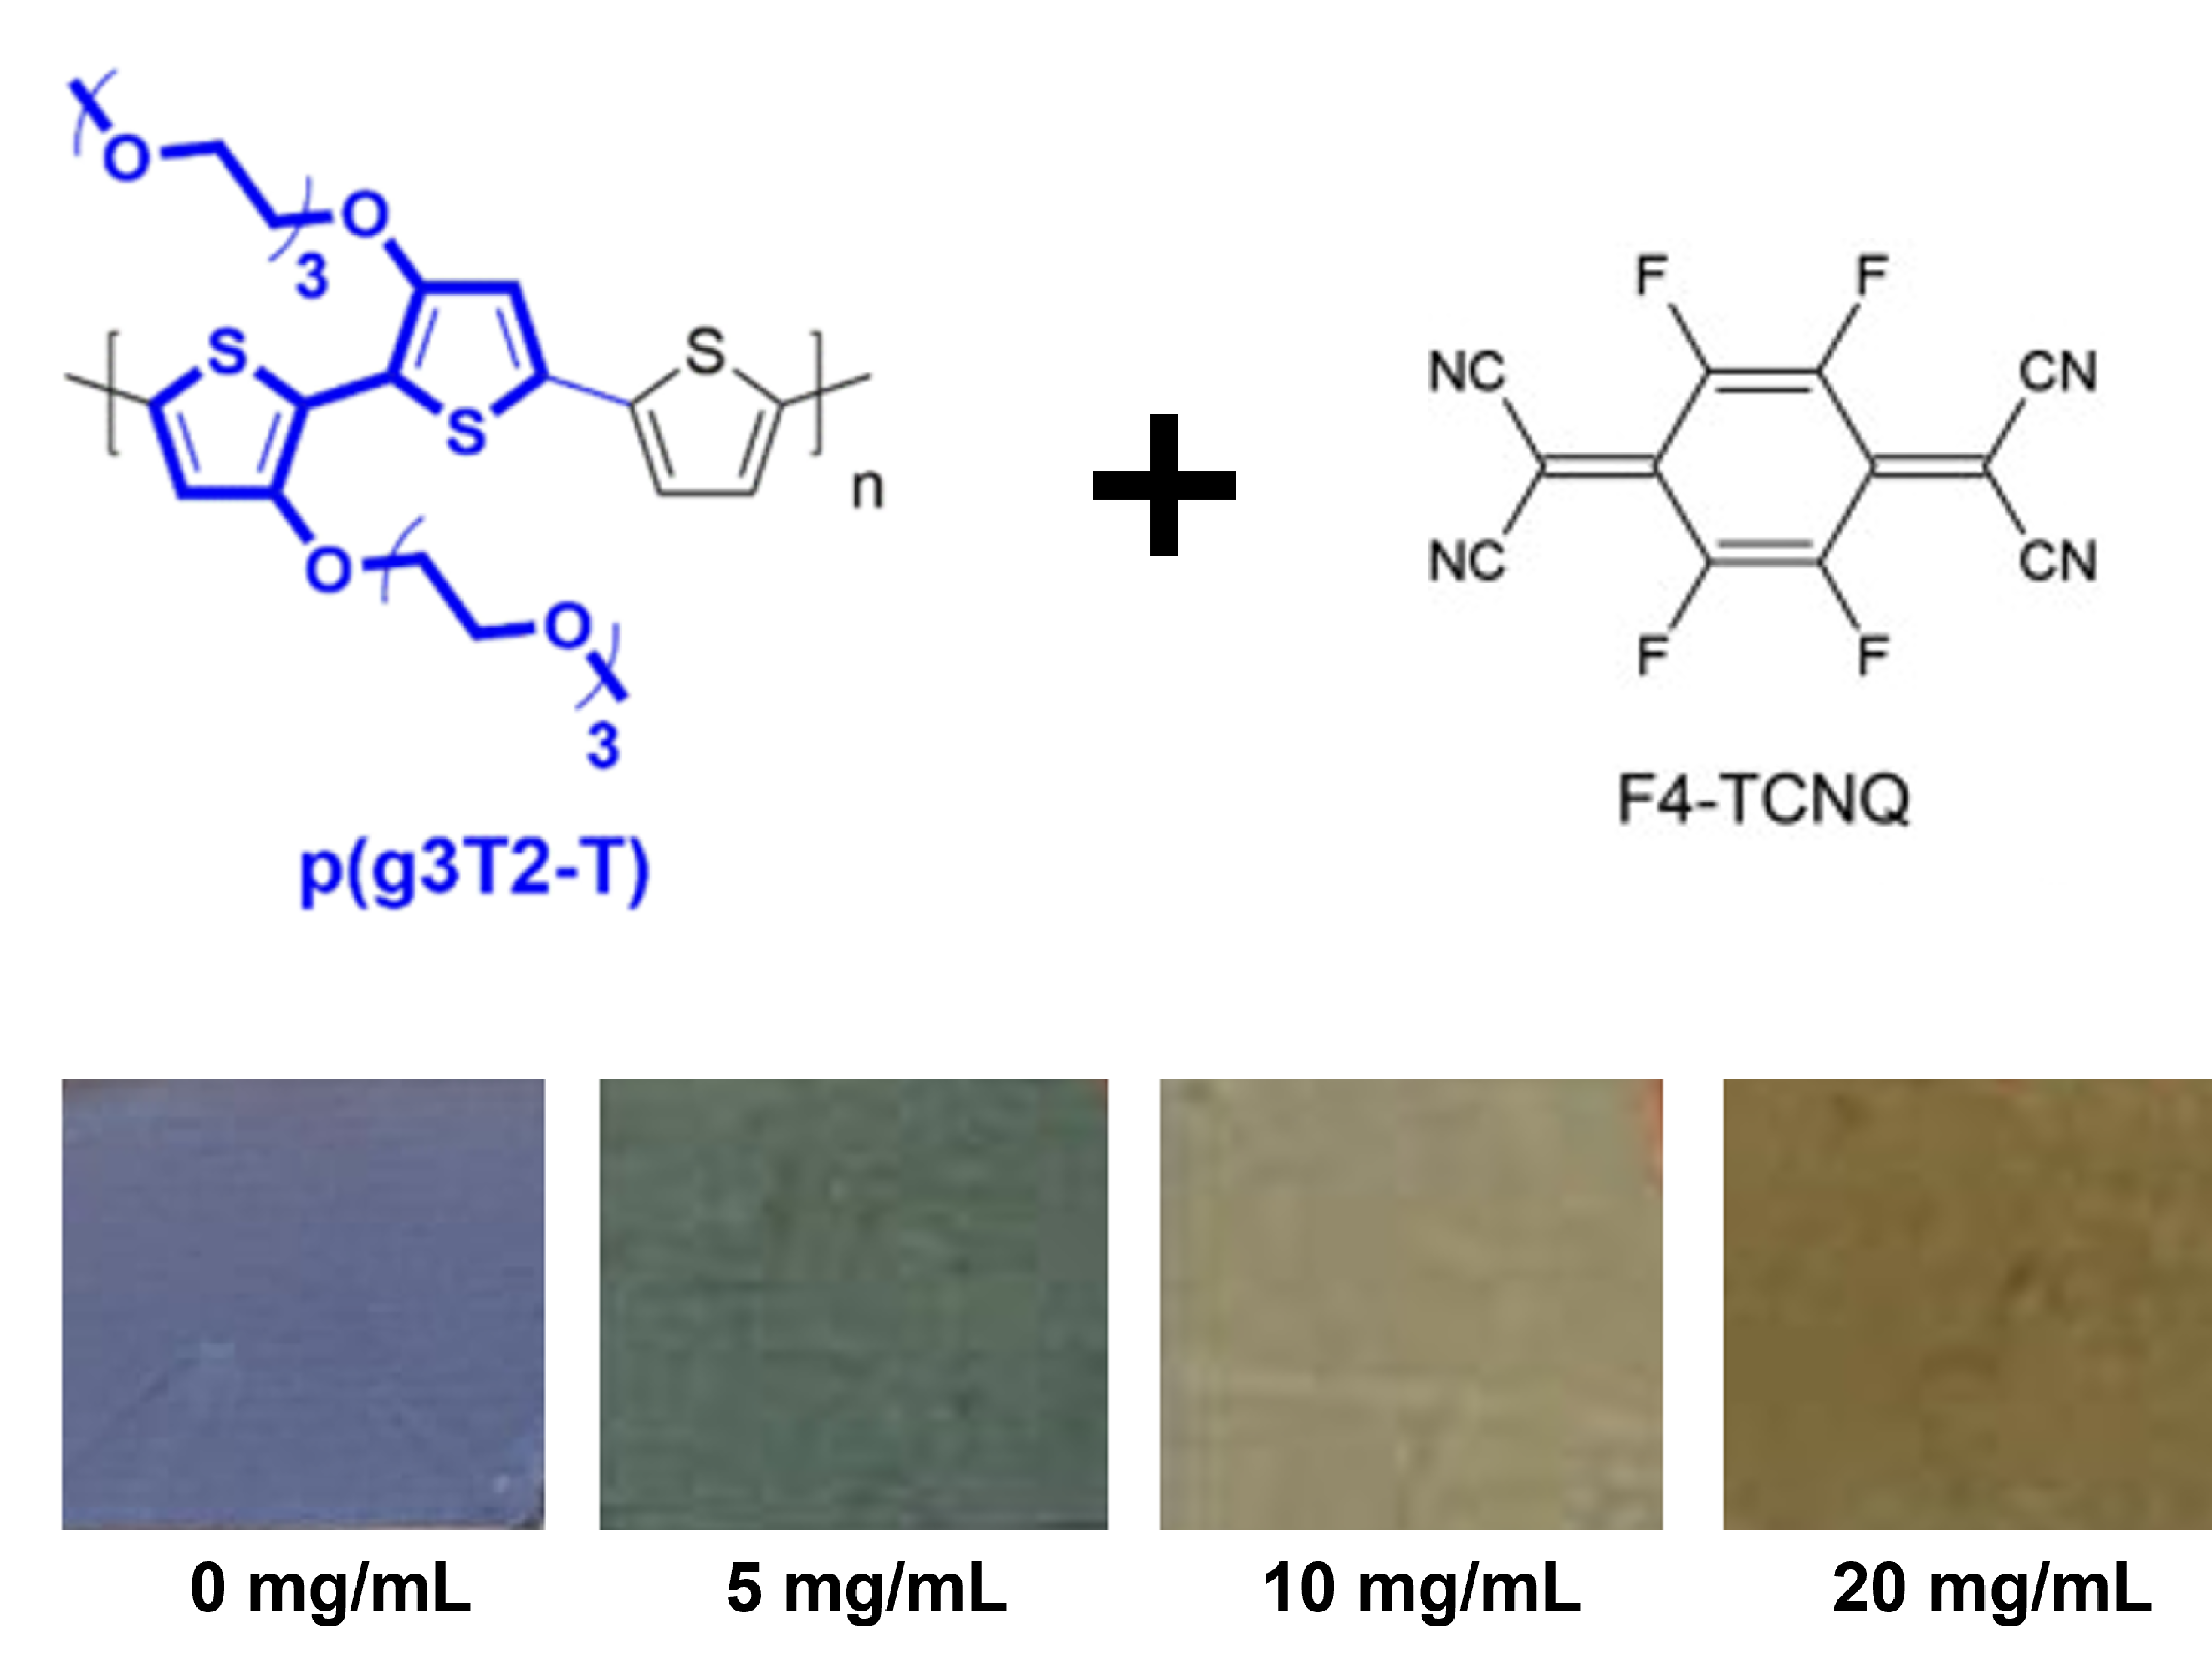
\includegraphics[width=8cm]{Images/pdf/doping_color.pdf}
  \caption[Color shift upon doping level increase]{(Top) Chemical structure of p(g3T2-T) and F$_{4}$TCNQ dopant. (Bottom) Color change upon increasing dopant concentration from 0 to 20 mg/mL.}
  \label{fig:color}
\end{figure}

\subsection{Absorbance and Dopants Diffusion}
The visible color hue shift can be described quasi-quantitatively by the absorbance spectra of the samples, as seen in Figure \ref{fig:abs}, where the undoped-p(g3T2-T) shows a prominent absorption peak at 588 nm (red), which diminishes with doping, characteristic from oxidation, and it is more intense with higher doping levels. New absorption peaks are seen at around 860 nm, this is due to generation of polarons that lead to new optical transitions, as explained in section... from the Background chapter. Tan et al. described the apparition of new absorption peaks within 300 to 600 nm, the higher energetic (lower wavelength) one is generated by unreacted neutral dopant species (TCNQ$^{0}$), while the second is due to the new dopant anions (TCNQ$^{-}$), the latter induce charges in our polymer \cite{tanTuningOrganicElectrochemical2022}. It is shown also, that after some days of storage, the initially dominant peak of unreacted neutral dopants is now lower in intensity than the anions peak, suggesting that the dopants were still diffusing through the polymer along the days. 

\begin{figure}[ht]
  \centering
  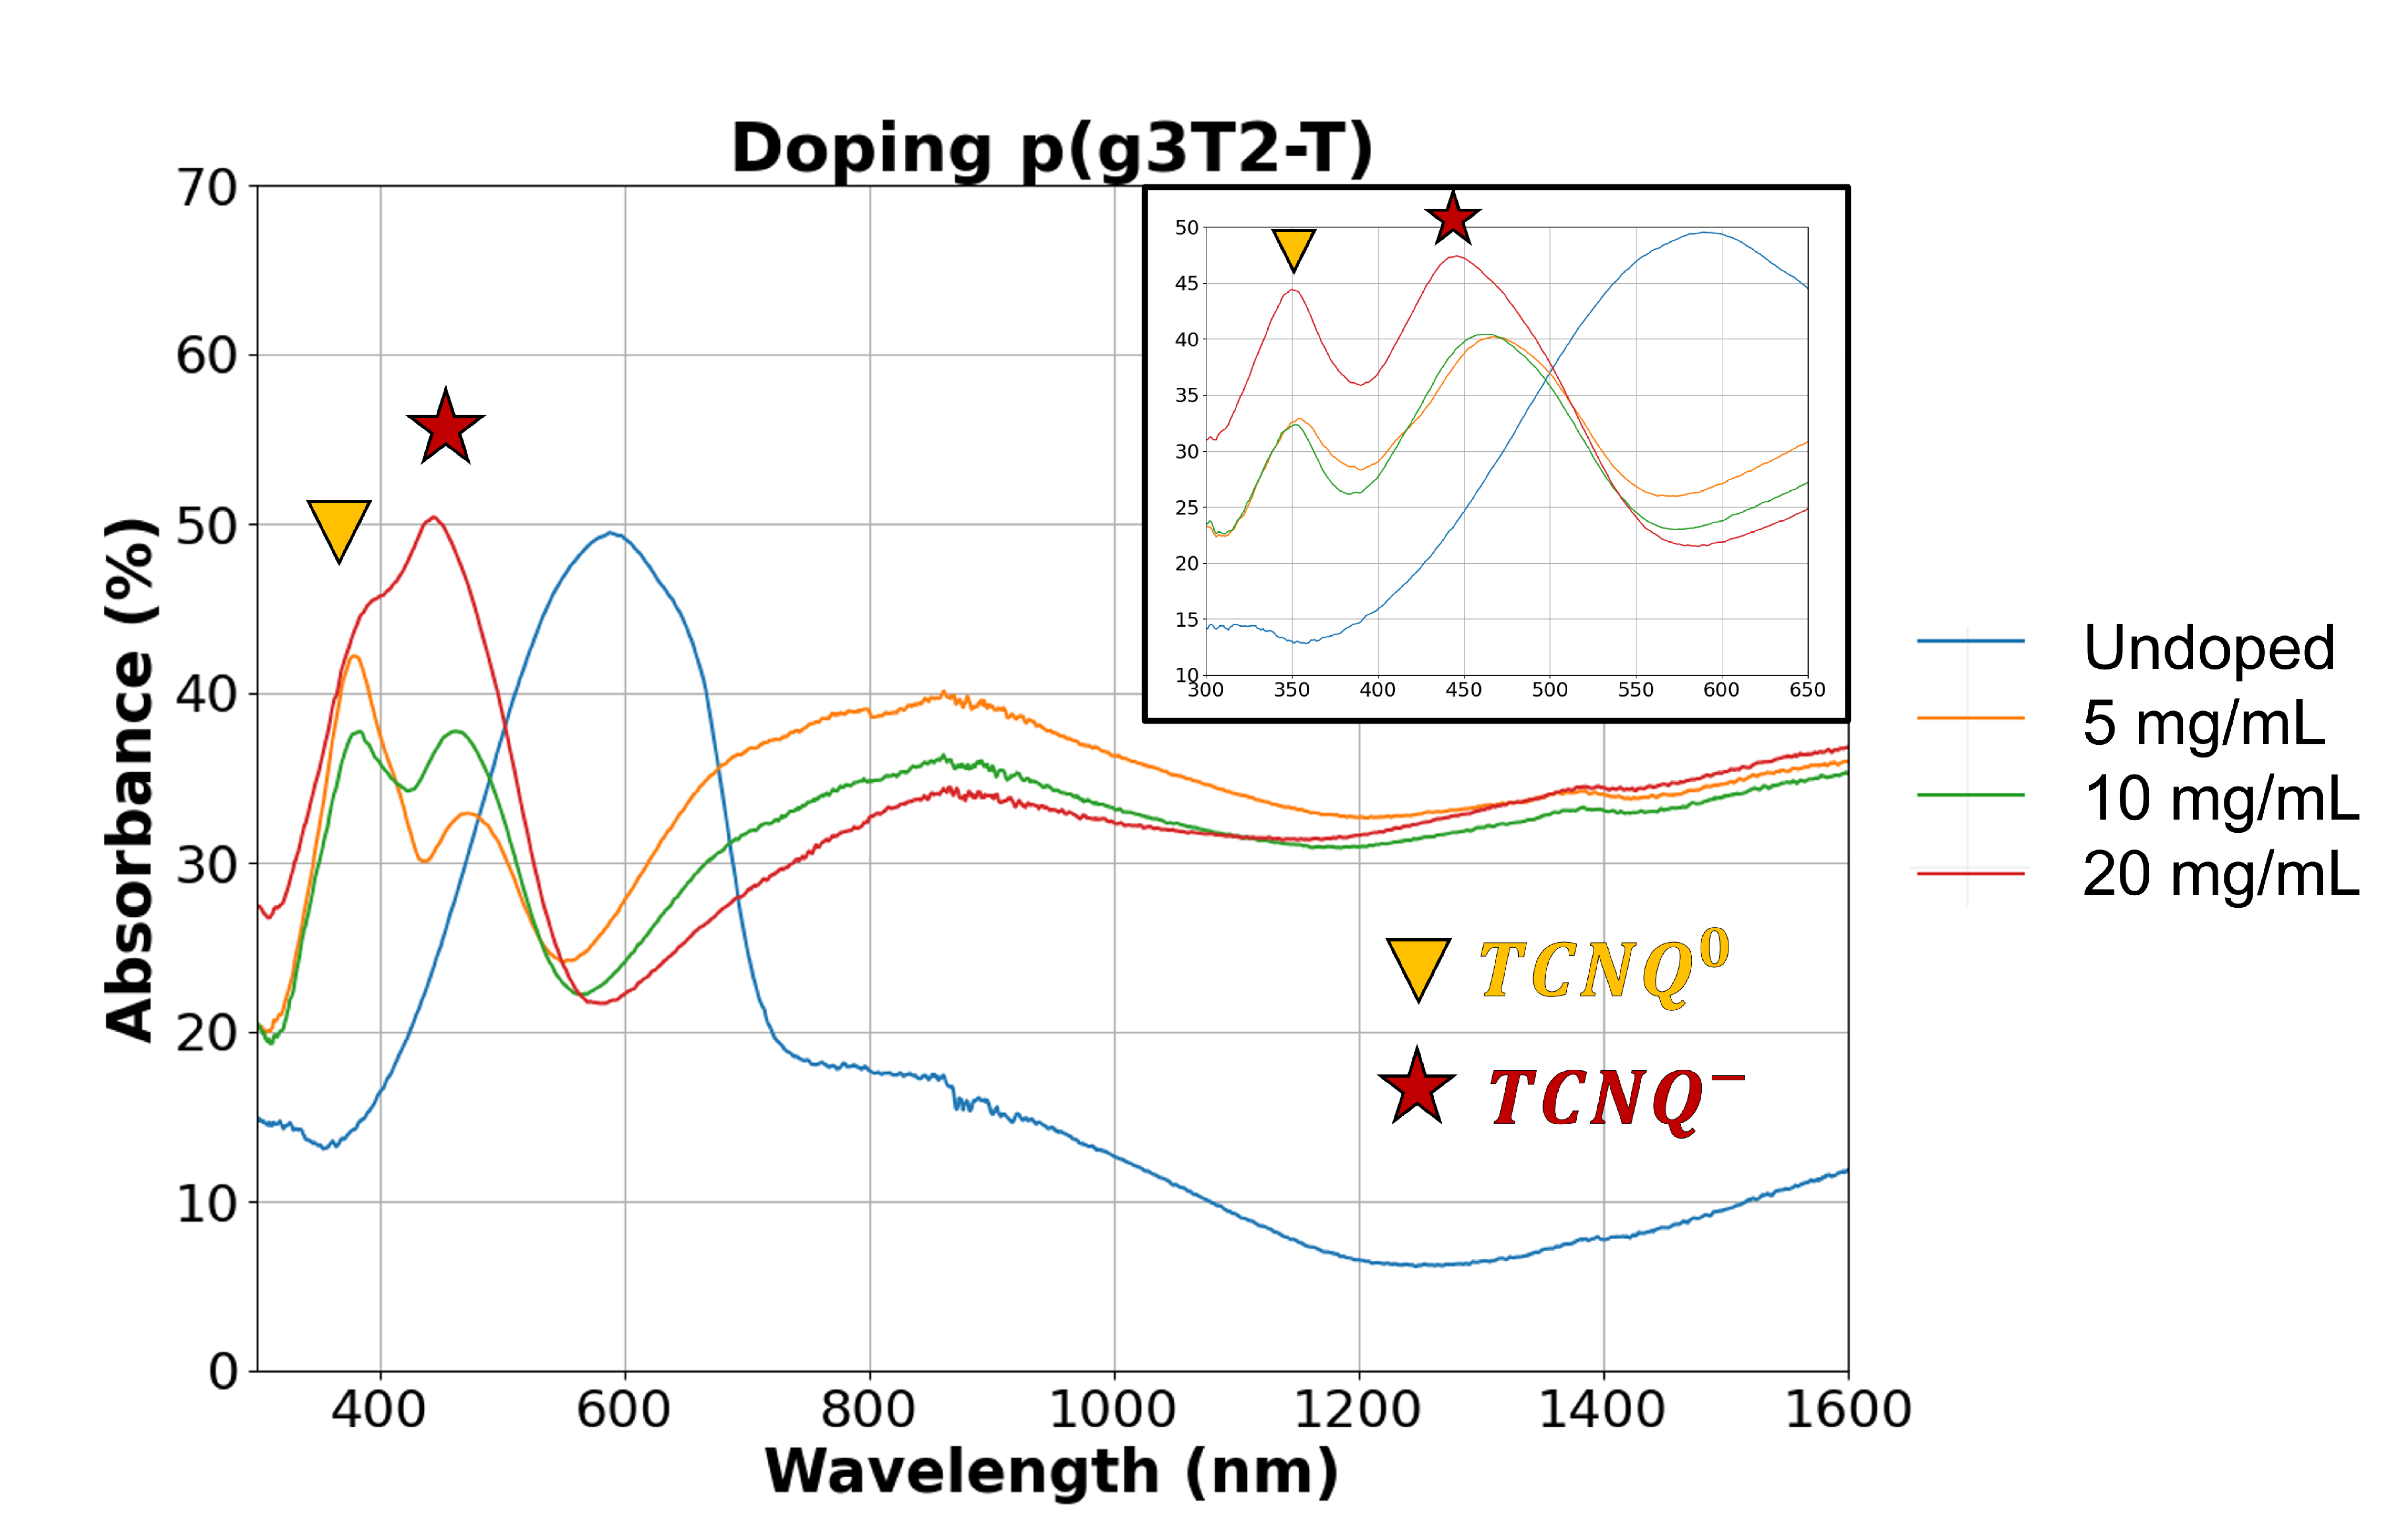
\includegraphics[width=\textwidth]{Images/pdf/abs+inlet.pdf}
  \caption[Absorbance spectra of different doping levels of p(g3T2-T)]{Spectra of undoped and doped-p(g3T2-T) at different doping levels, corresponding to samples on Figure \ref{fig:color}. Inlet represents absorbance after two weeks of storage in ambient conditions.}
  \label{fig:abs}
\end{figure}

Absorbance values are directly linked to the density of states of these new optical transitions \cite{bredasPolaronsBipolaronsSolitons1985}. From our spectra, the absorption value of the lowest doped-p(g3T2-T) (5 mg/mL) is higher (around 40\%), which may be counter-intuitive. However, as doping concentration increases, hence more electrons are taken out of the polymer chain, a bipolar is the energetically more favorable quasiparticle to generate. According to references \cite{tanTuningOrganicElectrochemical2022}\cite{enenglDopinginducedAbsorptionBands2016}, bipolaron formation is seen as a shift to lower energies in the broad absorbance the mid-IR region (wavenumber 1000-1600 cm$^{-1}$) so further analysis of hole bipolaron formation can be conducted with Fourier Transform InfraRed (FTIR) spectroscopy.
 
\subsection{Workfunction}

Although, the preparation of films for studying electron energy levels with UPS is ideally done under inert conditions to avoid any sort of contaminatio. The current fabrication process of OECTs inevitable exposes our films at ambient conditions. So measurements were taken following the deposition under ambient conditions. Yet, it is possible to distinguish an increase in the workfunction (shift of Fermi level) of the polymer. The Fermi level shift towards the HOMO level is higher at higher dopant levels, as represented in Figure \ref{fig:ups}, characteristic of p-type doping. Some possible additional contamination did not allow to measure sample with 20 mg/mL of dopant, but tendency is evident.

\begin{table}[ht]
\centering
\caption{Workfunction calculation from UPS measurements.}
\begin{tabular}{l|c|c|c}
& Undoped & 5 mg/mL & 10 mg/mL \\\hline
E$_{HBEC}$ [eV] & 17.35 & 16.47 & 16.36\\
E$_{HOMO}$ (vs E$_{F}$) & 4.28 & 3.27 & 3.24\\
WF [eV] & 3.87 & 4.28 & 4.86\\\hline
\end{tabular}
\label{tab:ups}
\end{table}

It is important to consider that UPS is a surface sensitive measurement, the penetration depth of the ultraviolet range electrons are around 2 nm, which is significantly lower than our polymer thickness (around 70 nm). So this technique limits our understanding of the dopants diffusion through the whole volume of the polymer. Although, we had some insights of this topic from the previous section, further analysis could be done with X-Ray Photoelectron Spectroscopy that has a higher penetration depth (around 5 nm), again also limited. %but along with depth profiling mode 

\begin{figure}[ht]
  \centering
  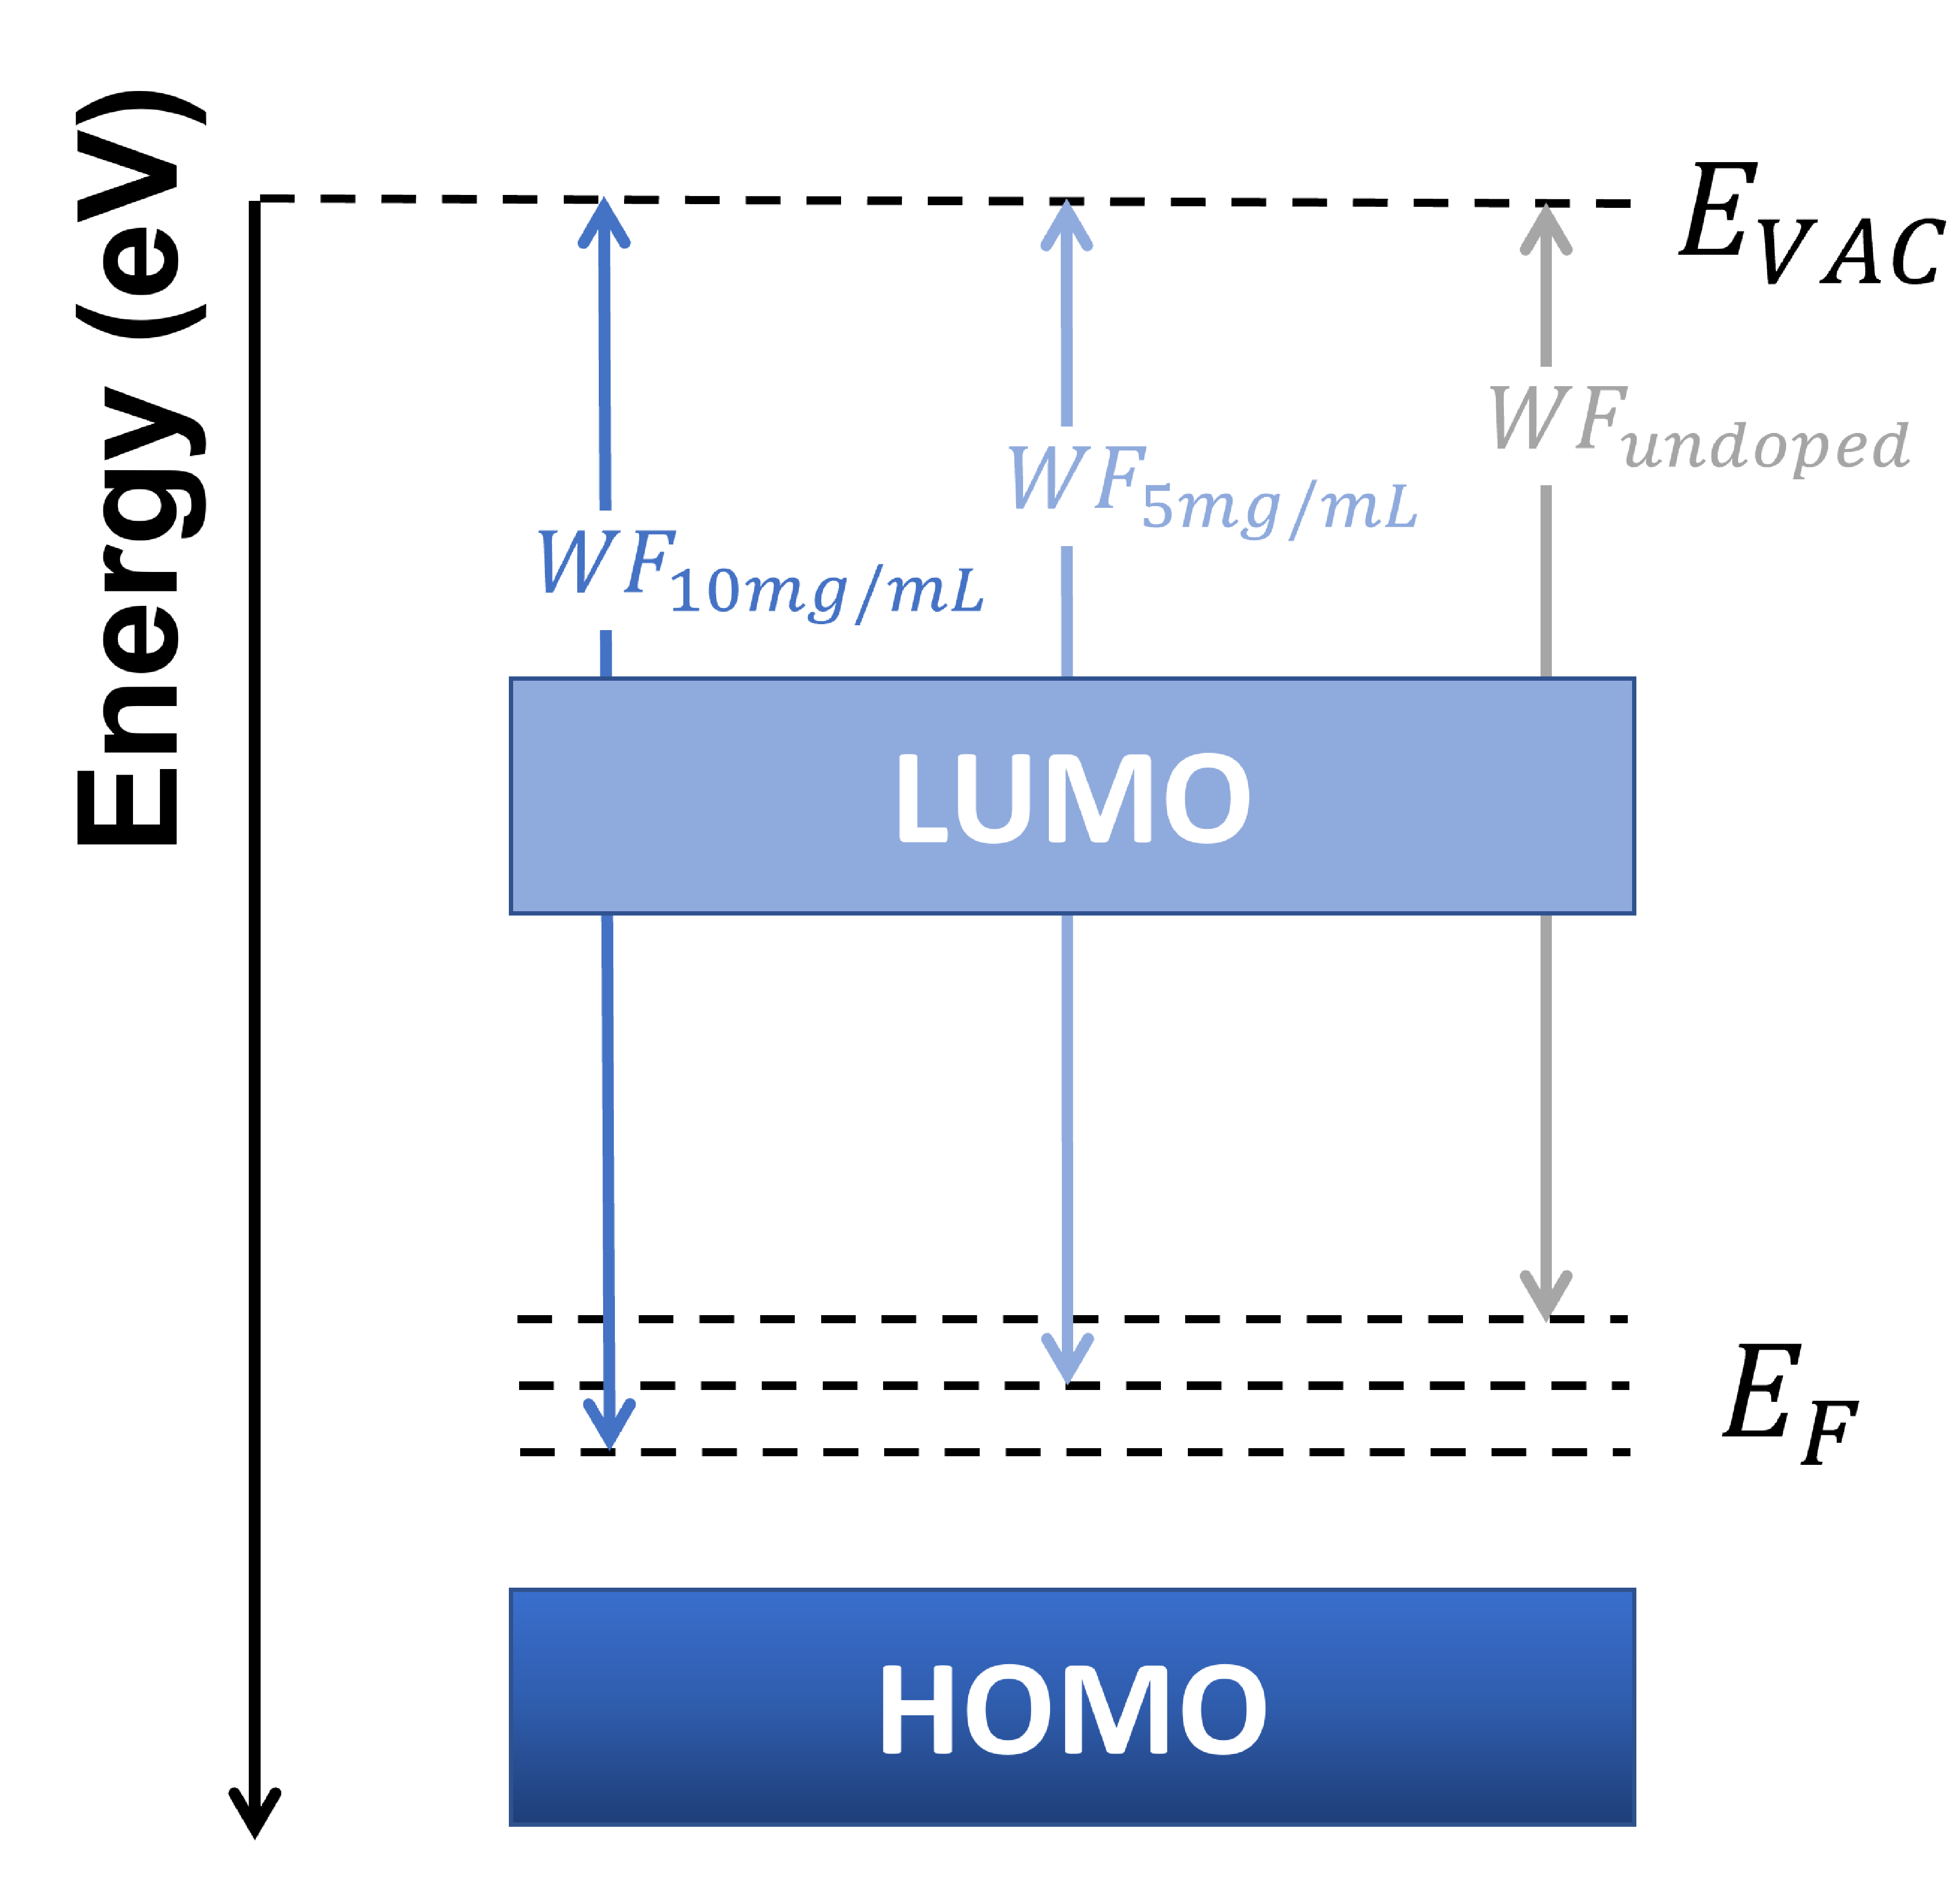
\includegraphics[width=8cm]{Images/pdf/WF.pdf}
  \caption[Representation of the Fermi level shift upon doping]{Representation of the Fermi level shift for doped-p(g3T2-t)}
  \label{fig:ups}
\end{figure}

\subsection{Thickness, Sheet Resistance and Resistivity}

Sheet resistance and resistivity shown in Table \ref{tab:res} were calculated using equations \ref{eq:rs} and \ref{eq:resist}, respectively, described in previous chapter. The film thickness was obtained with profilometer measurements, yielding to approximate 70 nm.

\begin{table}[ht]
\centering
\caption{Sheet resistance and resistivity calculations for undoped and doped films of p(g3T2-T)}
\begin{tabular}{l|c|c|c|c}
& Undoped & 5 mg/mL & 10 mg/mL & 20 mg/mL \\\hline
Sheet resistance ($\Omega$/sq) & 6.3M & 104.6k & 70.7k & 49.4k\\
Resistivity ($\Omega$cm) & 44.1 & 0.73 & 0.49 & 0.35\\\hline
\end{tabular}
\label{tab:res}
\end{table}

Upon doping there is a major decrease in both parameters, which is not as significant when adding more dopants, as seen in Figure \ref{fig:rho}. However, if comparing the decrease among doped samples, we could perceived a linear dependency upon increasing the dopant concentration. 

\begin{figure}[ht]
  \centering
  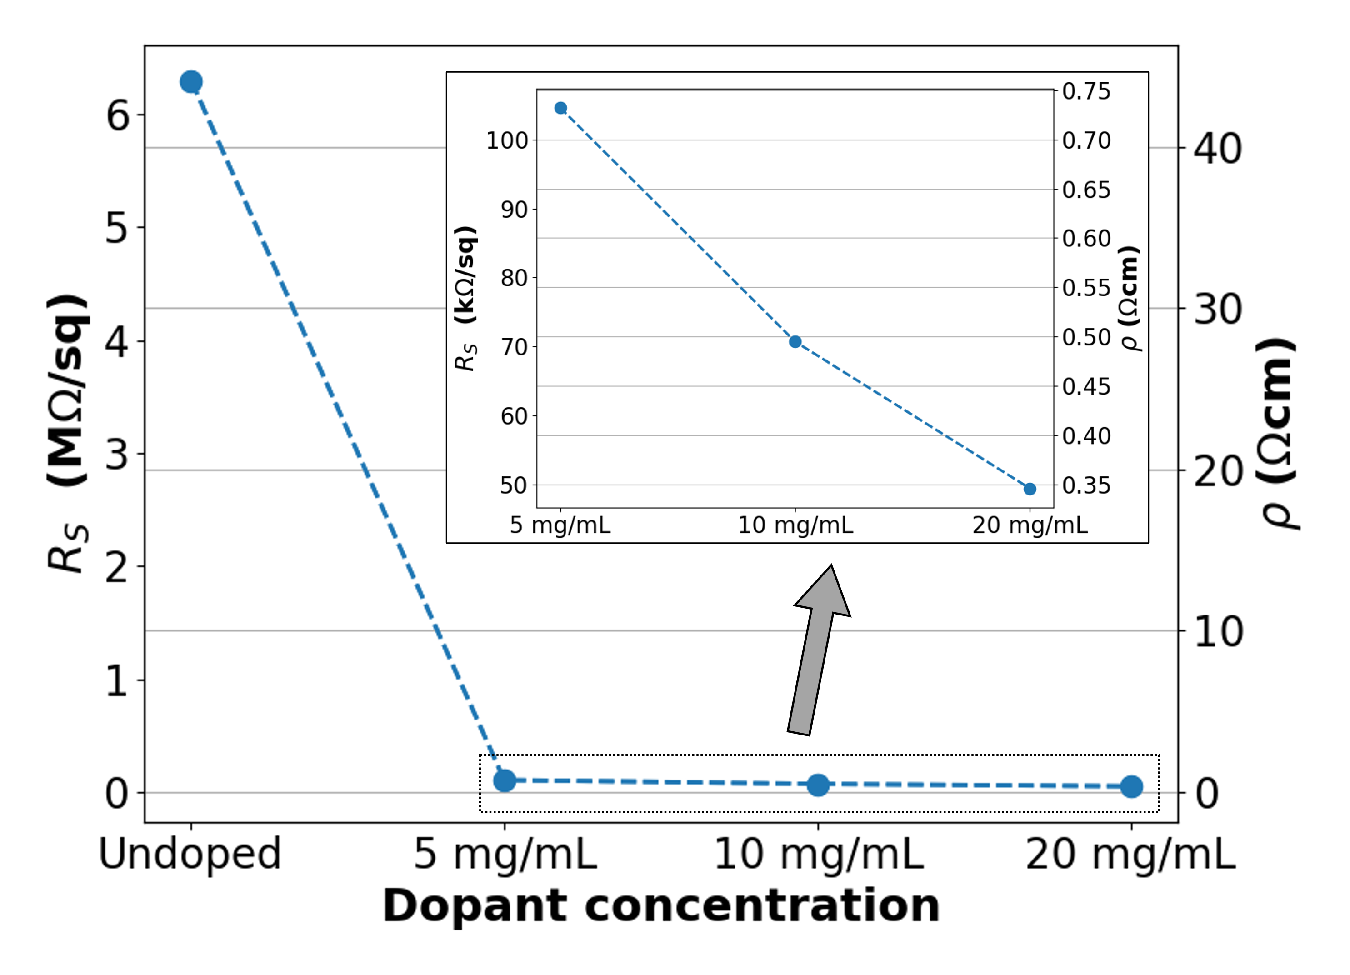
\includegraphics[width=10cm]{Images/pdf/resist+inlet.pdf}
  \caption[Sheet resistance and resistivity drop upon doping]{Sheet resistance and resistivity drop upon doping of p(g3T2-T). Inlet represents the quasi-linear drop of parameters as between doped samples.}
  \label{fig:rho}
\end{figure}

%\subsection{Roughness}

\section{Fabrication of Organic Electrochemical Transistors}

%Prior biasing gate, which is due to passive (ion) diffusion?

\subsection{Influence of Doping OECT Channel}
The fabrication process used a mask that include a microstructure gate, available for studying OECTs with channel and gate made of the same OMIEC material (commonly PEDOT:PSS). The result of the patterning process is shown in Figure \ref{fig:channel}. However, in this part, we are going to test only the OMIEC channel (p(g3T2-T) at different doping levels) with a non-polarizable gate such as Ag/AgCl pellet, using dropcasted solid-state electrolyte precursor to couple both channel and gate. Unfortunately, the sample that used solution with 20 mg/mL dopant concentration showed homogeneity issues that still allow photolithography but could not represent a fair comparison with the other devices, so it will be disregarded in this analysis.

\begin{figure}[ht]
  \centering
  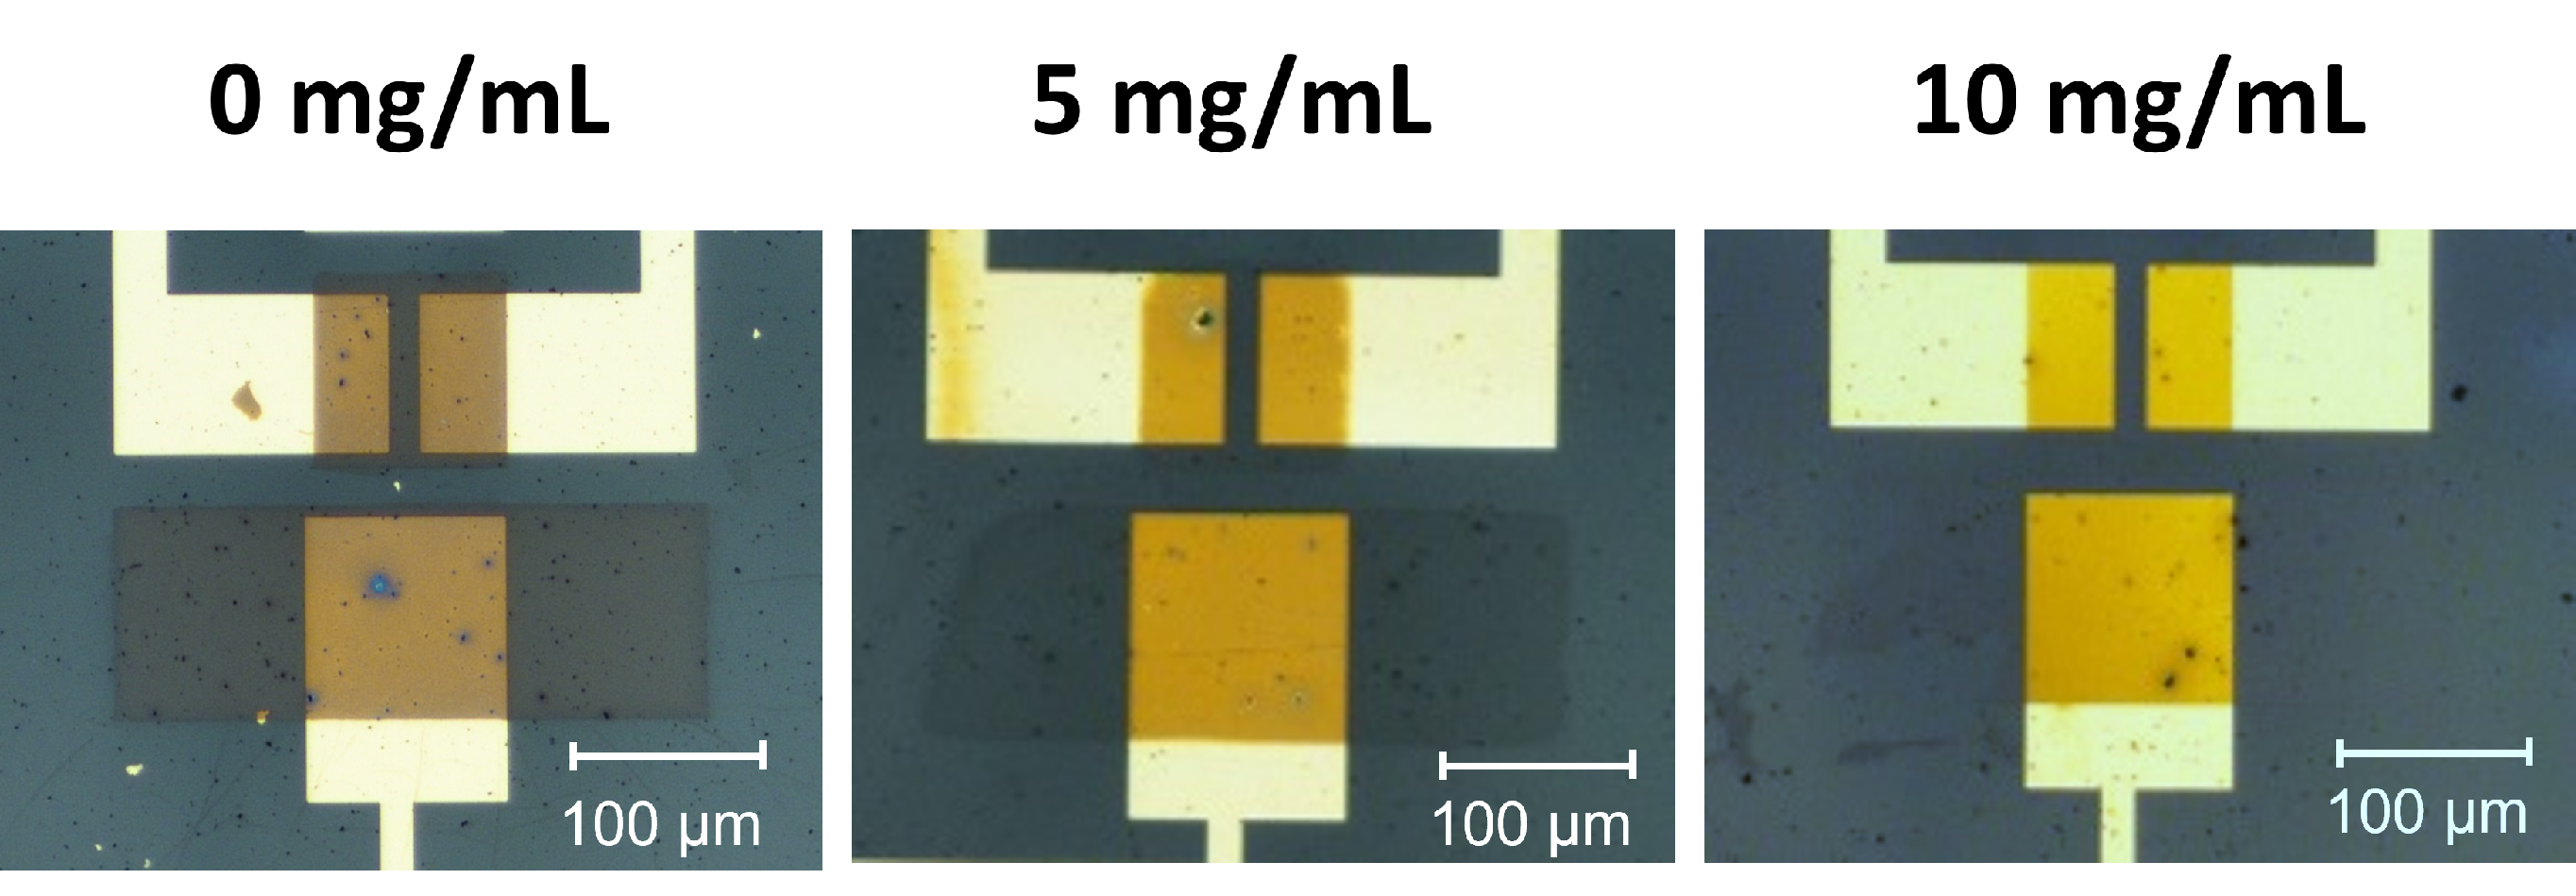
\includegraphics[width=10cm]{Images/pdf/BigGateDevices.pdf}
  \caption[Micrographs of a patterned channel and gate p(g3T2-T) at different doping levels]{Micrographs of patterned channel and gate with undoped, 5 mg/mL and 10 mg/mL doped p(g3T2-T) following procedures explained in Section \label{subsec:photo}.}
  \label{fig:channel}
\end{figure}

%U4 loop 2 as undoped pattern
%U2 loop 3 for doped 5
%U4 loop 3 for doped 10

\begin{figure}[ht]
    \centering
    \subfloat[]{{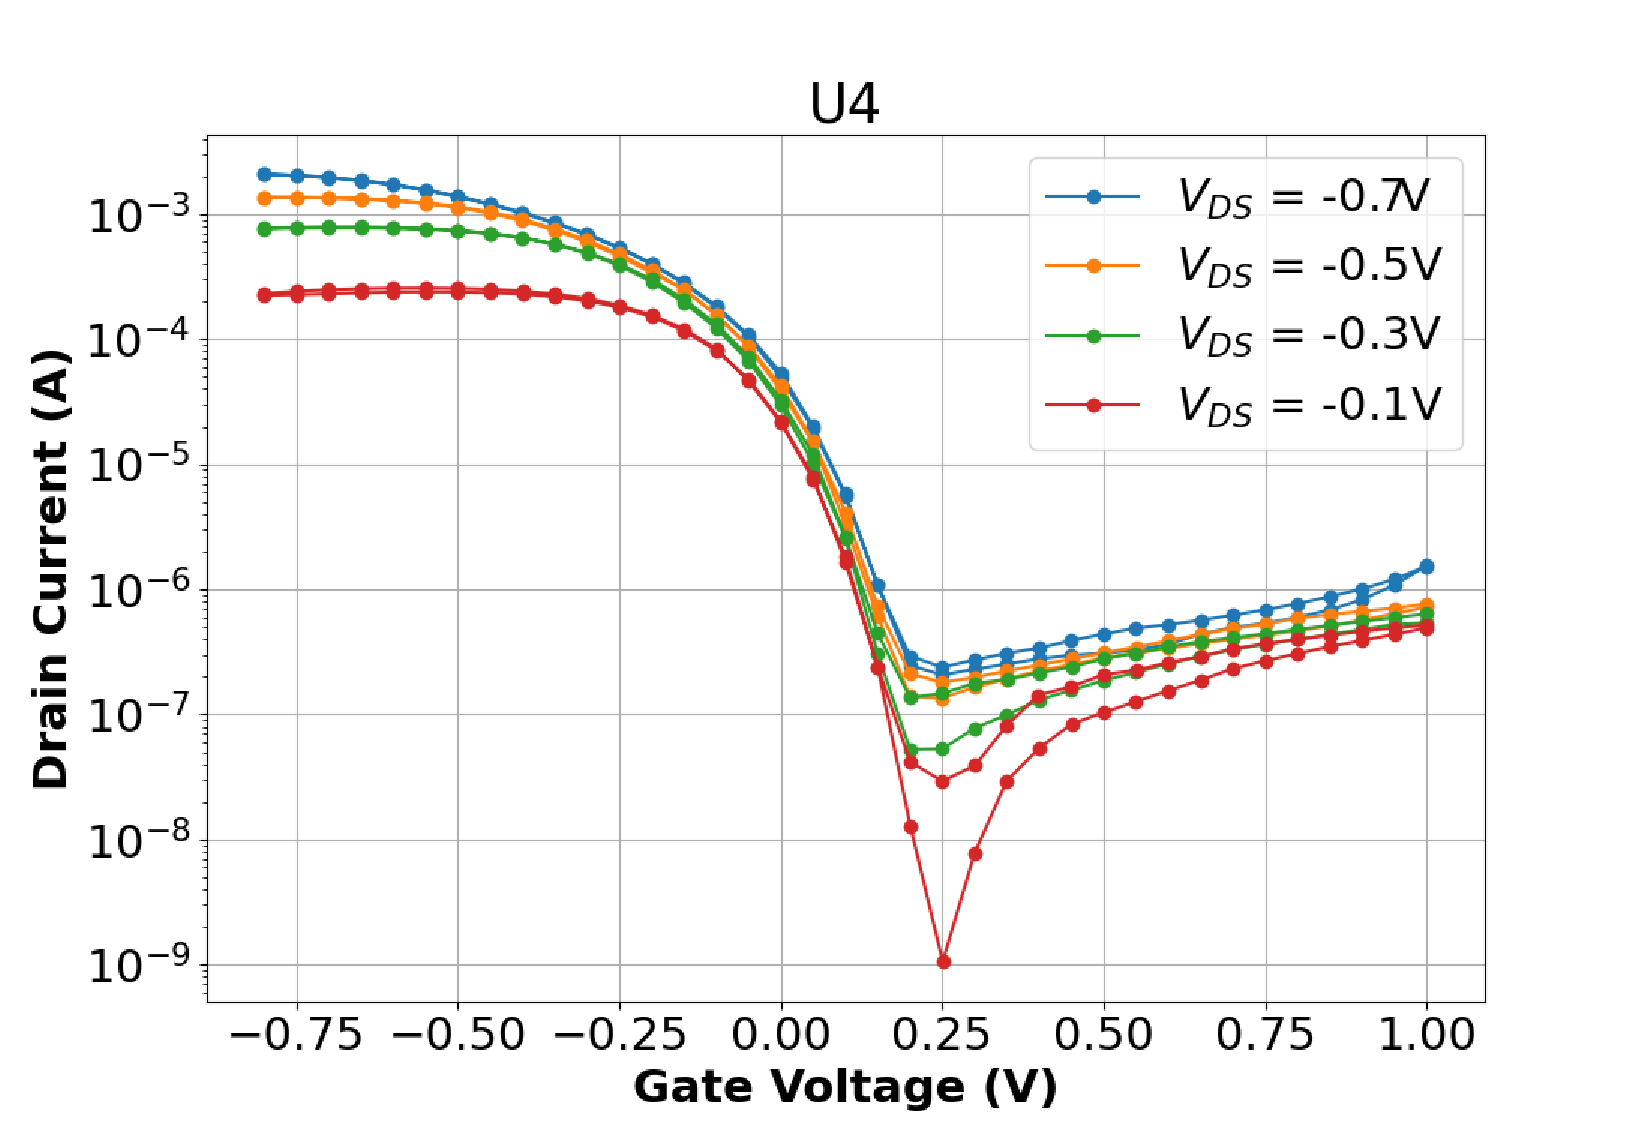
\includegraphics[height=5.5cm]{Images/pdf/transfer_undoped.pdf} }}
    \subfloat[]{{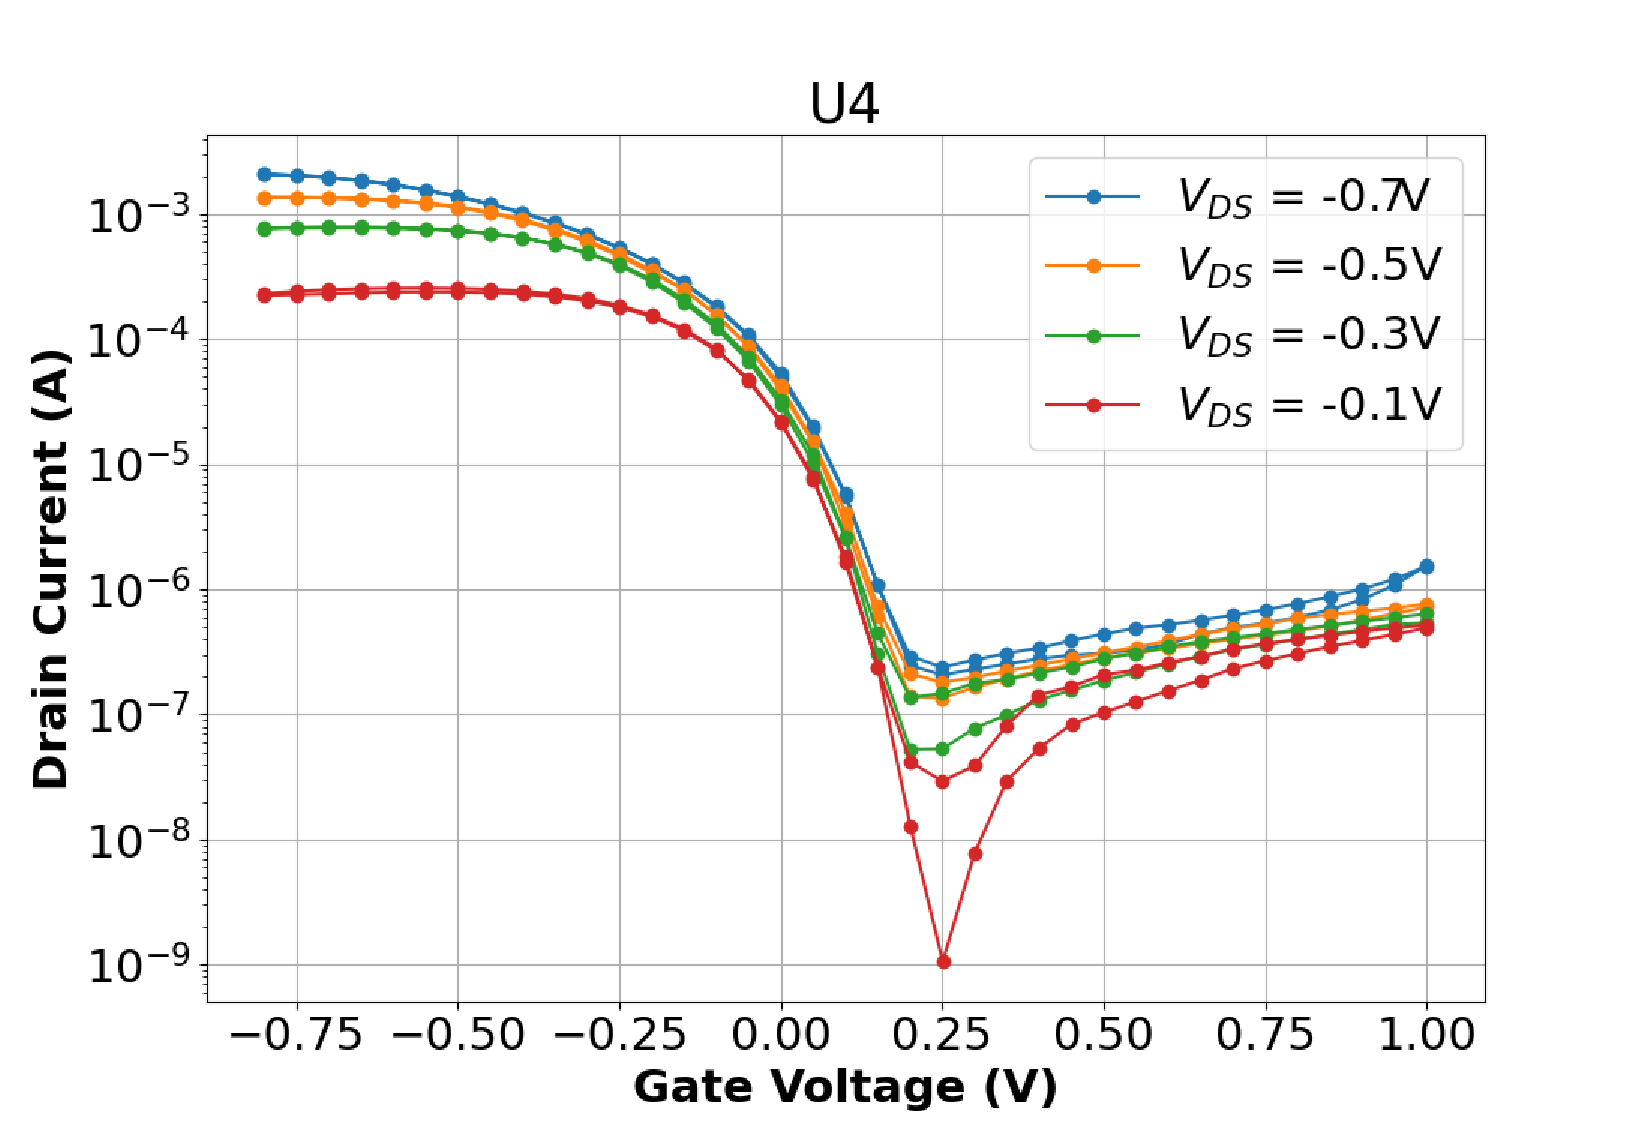
\includegraphics[height=5.5cm]{Images/pdf/transfer_undoped.pdf} }}
    \qquad
    \subfloat[]{{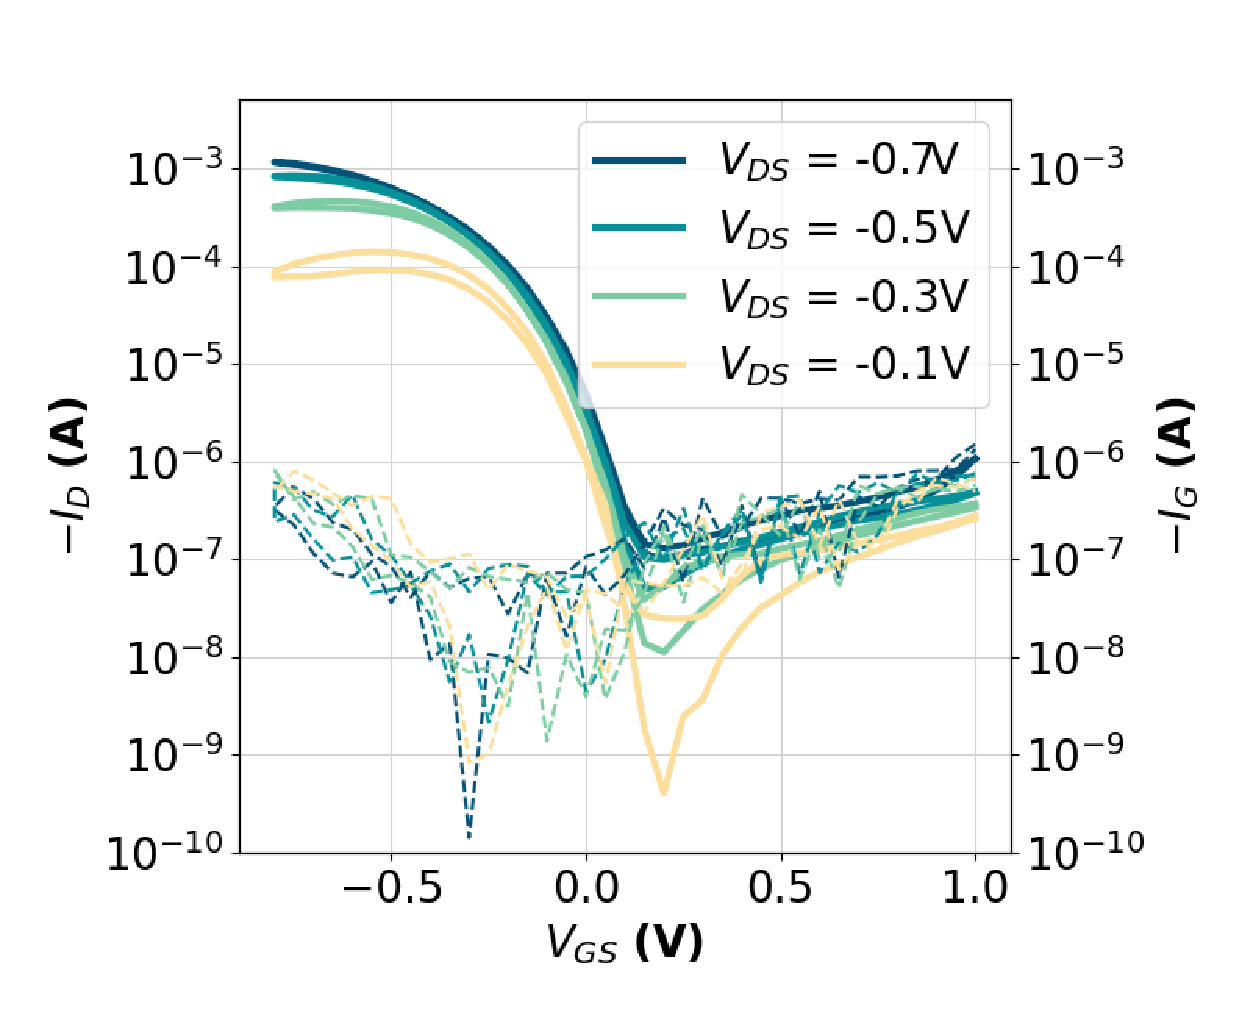
\includegraphics[height=5.5cm]{Images/pdf/transfer_doped5.pdf} }}
    \subfloat[]{{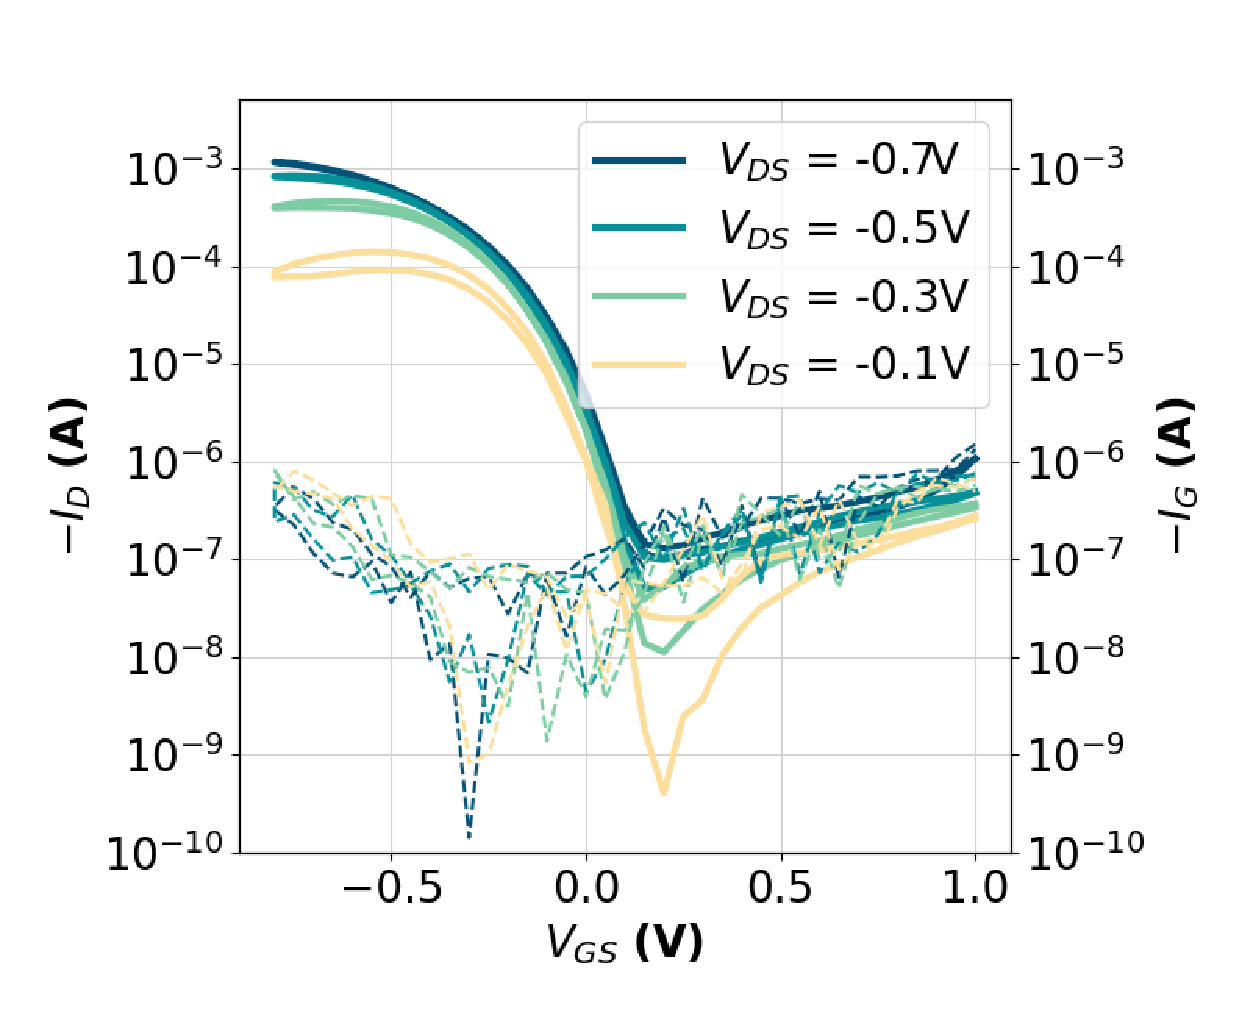
\includegraphics[height=5.5cm]{Images/pdf/transfer_doped5.pdf} }}
    \qquad
    \subfloat[]{{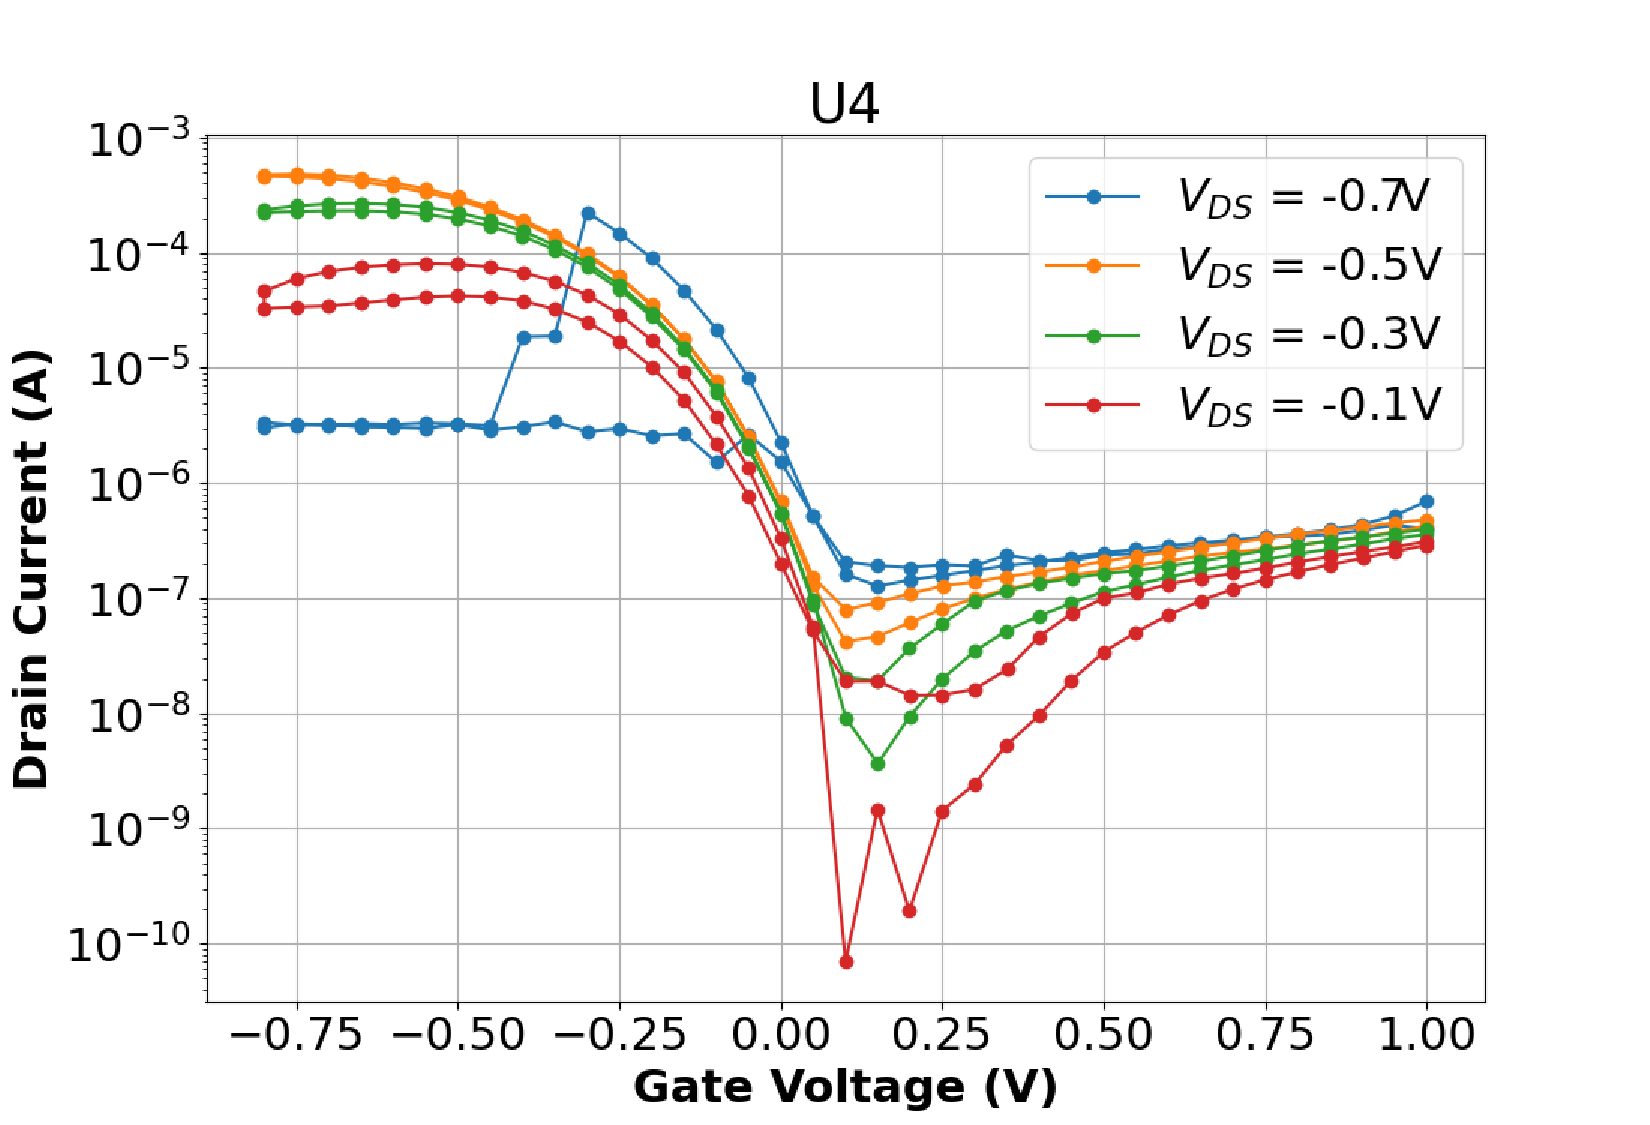
\includegraphics[height=5.5cm]{Images/pdf/transfer_doped10.pdf} }}
    \subfloat[]{{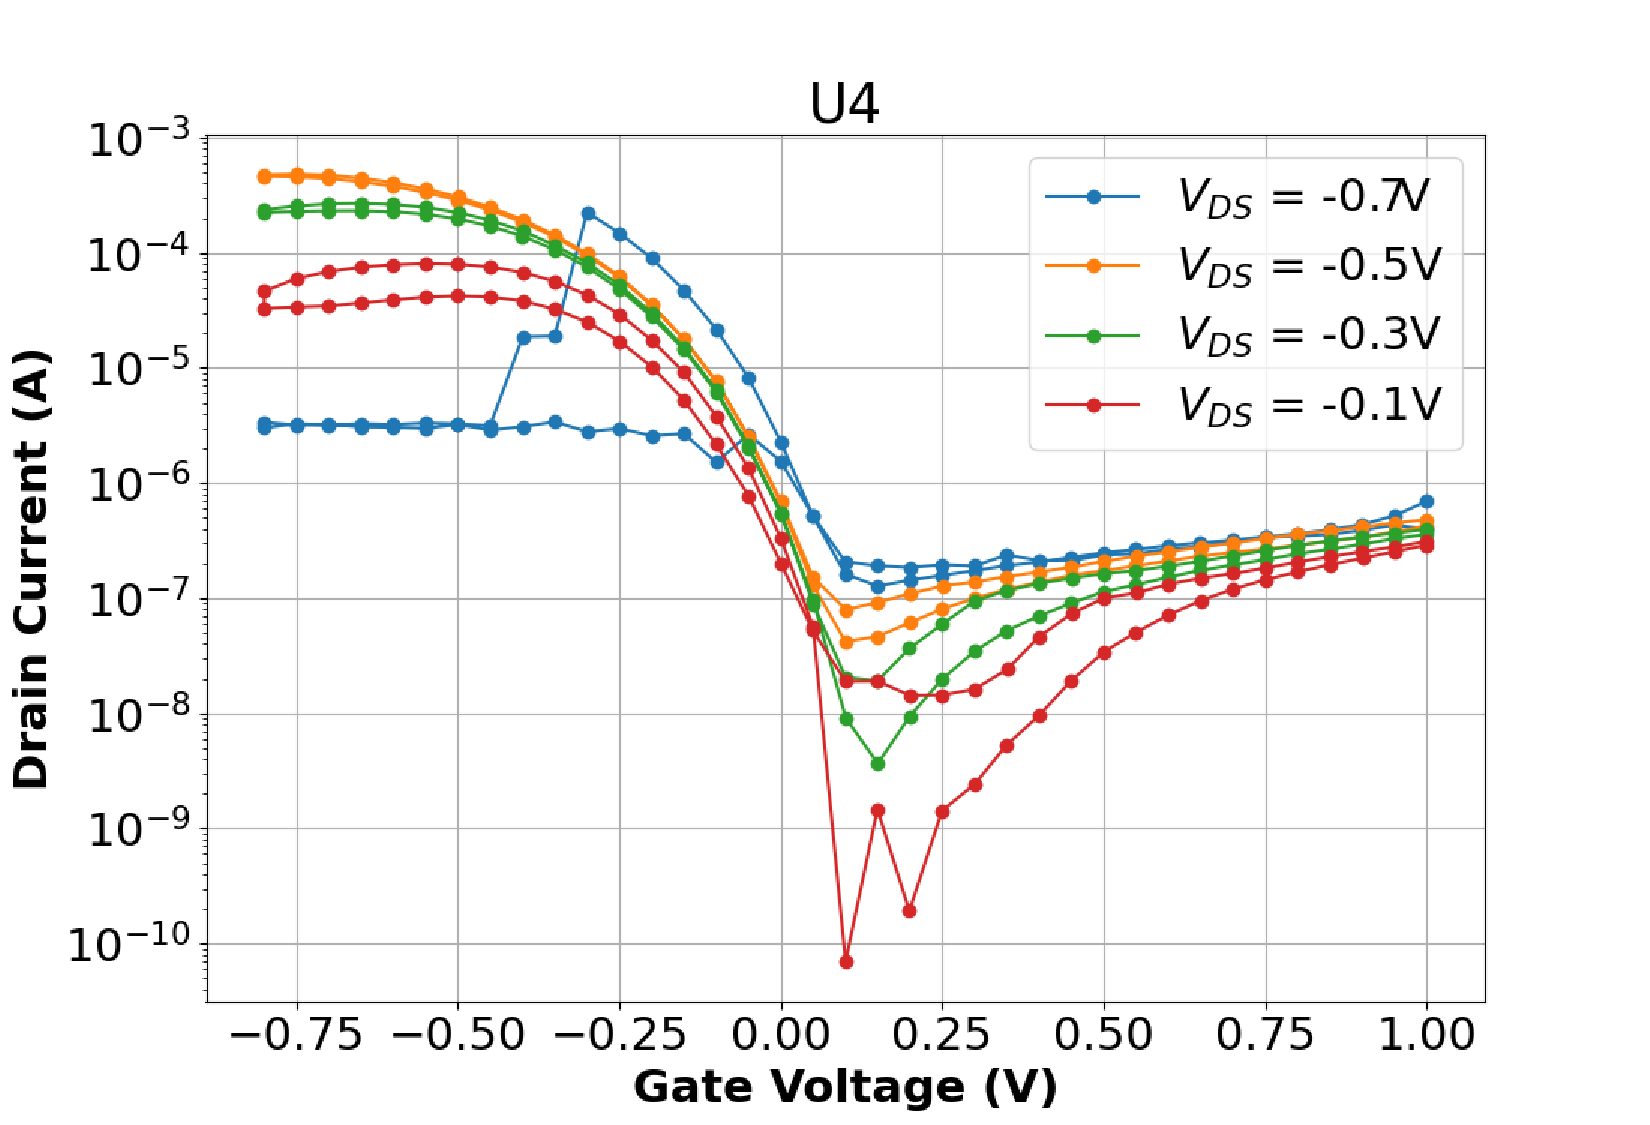
\includegraphics[height=5.5cm]{Images/pdf/transfer_doped10.pdf} }}
    \caption{Transfer characteristics and transconductance at different V$_{DS}$. a), c) and e) correspond to the exponential behavior of undoped, 5 mg/mL and 10 mg/mL doped, respectively.}
    \label{fig:transfercurves}
\end{figure}

\begin{table}[ht]
\centering
\caption{Maximum transconductance and $\mu$C* product calculation}
\begin{tabular}{l|c|c|c}
& Undoped & 5 mg/mL & 10 mg/mL \\\hline
g$_{m,max}$ [mS] & 17.35 & 16.47 & 16.36\\
$\mu$C* [Fcm$^{-1}$V$^{-1}$s$^{-1}$] & 4.28 & 3.27 & 3.24\\\hline
\end{tabular}
\label{tab:fom}
\end{table}


\subsection{Stability on Air of p(g3T2-T)}

\subsection{Reverse Oxidation of Undoped-p(g3T2-T}

\subsubsection{By Electrochemical Dedoping}

\subsubsection{By Heating}


\subsection{Solid-OECTs using Undoped p(g3T2-T)}


%The Ag/AgCl gate electrode’s work function is reasonably constant, the work function of an OMIEC gate electrode however may vary depending on its processing history and redox reactions with other species present in the electrolyte (e.g. molecular oxygen).28 Applying VGS only determines the potential difference between the gate and channel but does not control the potentials of either electrode (hence the position of the Fermi level) with respect to a reference. This leads to many challenges in operating an OECT with OMIEC gate electrodes.


\subsubsection{Dropcasted Solid-State Electrolyte}

\subsubsection{OECT with Dropcast Solid-State Electrolyte}

\subsubsection{OECT with Photopatternable Solid-State Electrolyte}

\subsubsection{OECT with Inkjet-Printed Solid-State Electrolyte}


\subsection{Solid-OECTs using Doped-p(g3T2-T)}

\begin{figure}
  \centering
  \includegraphics[width=10cm]{Images/pdf/dopingprocess.pdf}
  \caption[Energy diagram of p(g3T2-T) and dopants F$_{6}$TCNNQ and F$_{4}$TCNNQ]{Energy diagram of p(g3T2-T) with a) F$_{6}$TCNNQ and b) F$_{4}$TCNNQ. Ionization potential of p(g3T2-T) extracted from reference \cite{tanTuningOrganicElectrochemical2022} and electron affinities of the neutral species (EA$^{0}$) and of the anion (EA$^{-}$) of the dopants are extracted from cyclic voltammetry measurements in reference \cite{kieferDoubleDopingConjugated2019}.}
  \label{fig:doping}
\end{figure}

%Achieving effective charge transfer between the analyte and OMIEC requires appropriate alignment of the electrochemical potential of electrons on the OMIEC electrode and the redox specie. Failure to do so may result in the subsequent transfer of charges to other redox-active sinks in the environment, leading to undesirable side reactions and products that may interfere with the OMIEC’s operation. Electrons flow from a region of higher to lower electrochemical potential. Hence, achieving electron transfer from redox-active species to the OMIEC requires the latter to have a deep LUMO (high electron affinity) \cite{tanMixedIonicElectronic2022} %paper

%\section{Conclusion}
%\lipsum[86-88]

%%% Local Variables: 
%%% mode: latex
%%% TeX-master: "thesis"
%%% End: 
